\documentclass{article}
\usepackage[a4paper, tmargin=1in, bmargin=1in]{geometry}
\usepackage[utf8]{inputenc}
\usepackage{graphicx}
\usepackage{parskip}
\usepackage{pdflscape}
\usepackage{listings}
\usepackage{hyperref}
\usepackage{gensymb}
\usepackage{amsmath}
\usepackage{float}

% \usepackage{setspace}

% \renewcommand{\floatpagefraction}{0.9}


\newcommand\Problem[1]{
  \\
  \textbf{Q#1.}
}
\newcommand\Sol[1]{
  \\
  \textbf{A#1.}
  \\
}

\newcommand\Probsub[2]
{
  \\
  \textbf{Q#1.#2}
}

\newcommand\Solsub[2]
{
  \\
  \textbf{A#1.#2}
  \\
}

\newcommand\tab[1][0.5cm]{\hspace*{#1}}

\title{CMU Airlab Problem Statement}
\author
{
  Arka Sadhu - 140070011\\
  3rd Year Btech. Electrical Engineering
}
\date{December 2016}

\begin{document}
\maketitle

\section*{Problem Statement for Q2}
\Problem{1} Name one advantage and one disadvantage of using Euler angles (e.g. Roll-Pitch-Yaw), unit quaternions, rotation matrices and axis/angle representations of rotations.
\Sol{1}
\begin{itemize}
\item Euler Angles:
  \begin{itemize}
  \item Advantages:

    \begin{itemize}
    \item Only 3 parameters need to be stored.
    \item It is more human understandable and good for decomposing rotations into individual degrees of freedom.
    \end{itemize}

  \item Disadvantages:
    \begin{itemize}
    \item Interpolation is difficult.
    \item There are ambiguities in the order of Matrix Rotations.
    \item If the middle rotation is by 90$\degree$, it results in a Gimbal Lock.
    \end{itemize}
  \end{itemize}
  
\item Unit Quaternions:
  \begin{itemize}
  \item Advantages:
    \begin{itemize}
    \item There is no ambiguity, no gimbal lock, and interpolation can be done using slerp, producing smooth rotations.
    \item It requires only 4 parameters to be stored.
    \item Even translations can be accomodated using Dual Quaternions.
    \item Computation is efficient for computers.
    \item Consecutive rotation is simply multiplication of two quternions.
    \end{itemize}

  \item Disadvantages:
    \begin{itemize}
    \item In general it is not easy to visualize Quaternions, and need to be converted to Axis Angle Representation.
    \item The Quaternion-Algebra is quite involved.
    \item There exists redundancy, ie two quaternions may imply the same rotation.
    \end{itemize}
  \end{itemize}

\item Rotation Matrices
  \begin{itemize}
  \item Advantages:
    \begin{itemize}
    \item Rotations can be easily concatenated.
    \item They directly give the new axis of rotations, which may be required in some applications.
    \item With homogenous coordinates it is very easy to incorporate Translation too.
    \end{itemize}

  \item Disadvantages:
    \begin{itemize}
    \item Rotation Matrices need 9 parameters to be stored.
    \item The matrices must be orthogonal, and often due to floating point inaccuracy, they do not remain orthogonal, and the elements of the matrix may need to be recomputed.
    \end{itemize}
  \end{itemize}

\item Axis Angle Representation
  \begin{itemize}
  \item Advantages:
    \begin{itemize}
    \item Very easy to visualize.
    \item Can be very easily converted to quaternions.
    \end{itemize}
  \item Disadvantages:
    \begin{itemize}
    \item If $\theta = 0$ then axis is arbitrary.
    \item For $\theta$ and $\theta + 2*k*\pi$ produce the same result.
    \end{itemize}
  \end{itemize}
\end{itemize}

\Problem{2} Let $R^a = (\theta_{roll}^a, \theta_{pitch}^a, \theta_{yaw}^a)$ and $R^b = (\theta_{roll}^b, \theta_{pitch}^b, \theta_{yaw}^b)$ be a rotation corresponding to the following Roll-Pitch-Yaw angles (ZYX conventions):
$$\theta_{roll}^a = \pi/4 \hspace{2.5cm} \theta_{roll}^b = -\pi/3 $$
$$\theta_{pitch}^a = 0 \hspace{2.5cm} \theta_{roll}^b = 0 $$
$$\theta_{yaw}^a = \pi/3 \hspace{2.5cm} \theta_{roll}^b = 0 $$
Compute 3x3 rotation matrices corresponding to $R^a$ and $R^b$. Then compare $R^aR^b$ and $R^bR^a$ and give physical meaning to these two.
\Sol{2}
\[
  R^a =
  \begin{bmatrix}
    0.707107 & -0.353553 & 0.612372\\
 0.707107 & 0.353553 & -0.612372\\
        0 & 0.866025  &     0.5\\
  \end{bmatrix}
\]
\\
\[
  R^b =
  \begin{bmatrix}
          0.5  & 0.866025    &     0\\
-0.866025   &    0.5     &   -0\\
       -0    &     0     &    1\\
  \end{bmatrix}
\]
\\
\[
  R^aR^b =
  \begin{bmatrix}
    0.65974 & 0.435596 & 0.612372\\
    0.0473672 & 0.789149& -0.612372\\
    -0.75 & 0.433013   &    0.5\\
  \end{bmatrix}
\]
\\
\[
  R^bR^a =
  \begin{bmatrix}
    0.965926 &  0.12941 &-0.224144\\
    -0.258819&  0.482963& -0.836516\\
    0&  0.866025&       0.5\\
  \end{bmatrix}
\]
\\

We note that even though matrices are not commutative in general, they are associative. Let $R^{ab} = R^aR^b$. Clearly $R^{ab}$ is inturn a Rotation matrix. When $R^{ab}$ is applied to some other matrix,i.e. pre-multiplied to a matrix (say $R^{ab}*M$) the multiplication can be viewed in two steps, first multiplication with $R^b$ and then with $R^a$. Similarly with $R^{ba}$, the transformation can be viewed as successive rotations.

Since rotations in 3D are in general not commutative, here too, $R^{ab} \neq R^{ba}$.
\\
\Problem{3} Compute the quaternions $q^a$ and $q^b$ equivalent to the matrices $R^a$ and $R^b$ . Are these quaternions a unique representation of these rotations?
\Sol{3}
Representing Quaternions in the form of [w x y z]
\[
  q^a =
  \begin{bmatrix}
    0.800103 & 0.46194 & 0.191342 & 0.331414\\
  \end{bmatrix}
\]
\\
\[
  q^b =
  \begin{bmatrix}
    0.866025 &
       0 &
       0 &
    -0.5 \\

  \end{bmatrix}
\]
\\
For Quaternions we note that $q$ and $-q$ both give the same rotation. Hence these Quaternions are not a unique representation of these rotations. Other than this the relationship is unique.

\Problem{4} Compute two compositions of the rotations using quaternions, $q^c = q^aq^b$ and 
$q^d = q^bq^a$ . Are $q^c$ and $q^d$ the same? Compute the relative rotation between $q^a$ and
$q^b$ as $q^e = q^a(q^b)^{-1}$ . Then compute the composition $q^f = q^eq^b$ . Verify that $q^f$ and
$q^a$ are the same.
\Sol{4}
\[
  q^c =
  \begin{bmatrix}
    0.858616&
    0.304381&
    0.396677&
    -0.113039\\
  \end{bmatrix}
\]
\\
\[
  q^d =
  \begin{bmatrix}
    0.858616&
    0.495722&
    -0.0652631&
    -0.113039\\
  \end{bmatrix}
\]
\\
As expected $q^c$ and $q^d$ are not the same, since rotations in 3d are in general not commutative.
\[
  q^e =
  \begin{bmatrix}
    0.527203&
    0.495722&
    -0.0652631&
    0.687064\\
  \end{bmatrix}
\]
\\
\[
  q^f =
  \begin{bmatrix}
    0.800103&
    0.46194&
    0.191342&
    0.331414\\
  \end{bmatrix}
\]
\\
As expected $q^f = q^a$.

\Problem{5} How does axis/angle representation relate to quaternion? For example, how to
convert between quaternion q = (x, y, z, w) and angle/axis (n, θ)? Is the conversion
unique or not? If not, how many?
\Sol{5}
Considering the representation of the quaternion as $q = [v \tab s]$, where v is the complex part
and s is the scalar part. Therefore $v = [x \tab y \tab z]$ and $s = w$.

The axis angle and quaternions are closely related. Assumption is that the quaternion is a unit quaternion.
\begin{itemize}
\item Quaternion $[x y z w]$ to Angle Axis $(n,\theta)$:
  $$\theta = 2 * \cos^{-1} w$$
  $$n_x = \frac{x}{\sqrt{1 - w^2}}$$
  $$n_y = \frac{y}{\sqrt{1 - w^2}}$$
  $$n_z = \frac{z}{\sqrt{1 - w^2}}$$
\item Angle Axis to Quaternion:
  $$w = \cos \frac{\theta}{2}$$
  $$x = \sin \frac{\theta}{2}$$
  $$y = \sin \frac{\theta}{2}$$
  $$z = \sin \frac{\theta}{2}$$
\end{itemize}

Except for the fact that anti-podal Quaternions represent the same rotation there is no other ambiguity, i.e. $q$ and
$-q$ represent the same axis angle rotation. But this is to be expected since $(n,\theta)$ and $(-n,-\theta)$ also represent
the same rotation.

\Problem{6} Assuming Euler angles are small, it is very useful to know the approximation:
$R \approx I + [\omega]_×$ , where $[.]_x$ is the skew-symmetric operator and $\omega$ is the small rotation.
Now can you write down $\frac{\partial Rv}{\partial w}|_{\omega = 0}$ where $v \in R^3$
\Sol{6}
Given that $R \approx I + [\omega]_×$ we deduce : $$Rv \approx v + [\omega]_xv$$
$$Rv \approx v + \omega \times v$$
$$Rv \approx v - v \times \omega$$
$$Rv \approx = v - [v]_x\omega$$
Now we can differentiate easily, using the fact
$$\frac{d(a^Tx)}{dx} = a^T$$
Hence we get
$$\frac{\partial Rv}{\partial w}|_{\substack{\omega = 0}} = -[v]_x$$

\section*{Problem Statement for Q4 : 3D Perception}
\Problem{1} Plane Segmentation Tutorial
\Sol{1} Plane Segmentation is done using SAC segmentation. First the model type is selected as a plane, and then computation method is selected as RANSAC. The code basically chooses points which satisfy the equation of a plane, using RANSAC method. Once it has found the plane with maximum number of inliers,it computes the equation of the plane in the form $$ax + by + cz + d = 0$$. It then colors those points, and then removes all those inliers, and repeats the method to get a new set of inliers. This way red, green and blue points are shown.

The problem asked us to use display the normal vector arrows of the plane in the same colors as those belonging to the plane.

I have done this using the Marker Arrow. I have computed the centroid of the points in a particular plane, and chosen this point to show the arrow. I also had the model coefficients for the plane in the form of $$ax + by + cz + d = 0$$ and hence I knew the direction of the normal is $$v = (a,b,c)$$ I simply used the Eigen library to get the quaternion form of this using the function FromTwoVectors, which gave me the orientation in the quaternion form, and I used these values to set the orirentation of the marker arrow, and also set the color same as that of the points.

\begin{figure}[H]
  % \textbf{Title}\\
  \centering
  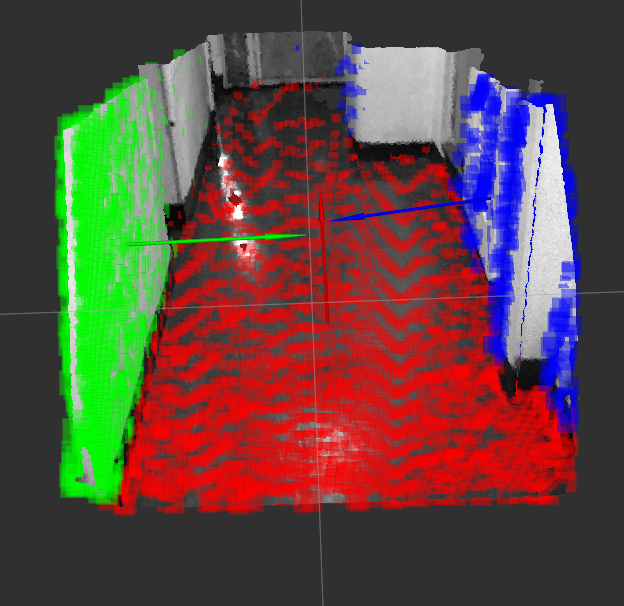
\includegraphics[scale=0.5]{images/rviz_screenshot_2016_12_29-11_25_46}
  \caption{Plane Segmentation Normal Vectors}
  \label{Fig:1}
\end{figure}

\Problem{2} 3D reconstruction with Stereo
\Sol{2} This was considerably tougher problem. The code was written following the guidelines provided in the problem statement. In brief the following steps were followed:
\begin{itemize}
\item Loading the data from data.json, left\_calib.json and right\_calib.json to the program. The default function recorded the filenames, and poses, which basically gives us Translation and Rotation in a matrix format. In addition to this, I also loaded the Translation and Rotation (in quaternion form) separately. 
\item 
\item For disparity map computation, a class \textbf{Disp\_map} is constructed, which stores the disparity map, a pointer for the Opencv implementation of Semi Global Block Matching (SGBM). The code for disparity computation is similar to that used in an example code in OpenCV cpp, for stereo matching. The disparity map is stored as a float. The class \textbf{Disp\_map} also has a funciton to store the disparity map in png format. Object oriented approach is used since it simplifies the code, and different algorithms can be implented.
\item After the disparity map is computed, another class \textbf{Depth\_map} is constructed which stores two point clouds generated from different computations, one using my implementation of reprojection and the other using default opencv implementation of reprojection. Both give similar point cloud results, but opencv implementation gives slightly better results. The class also includes methods to compute the transfomration of a point cloud, and methods to save the point clouds in pcd or ply format.
\item Once the point cloud is formed, it is saved in PCD format. The point cloud has several artifacts at places with ambiguous textures.
\item Transformation into the same coordinate system is done using the pcl implementation of \textbf{tranformPointCloud}. Concatenation of point clouds is simply adding all the transformed point clouds, which is trivial. The resulting point cloud is also saved.
\end{itemize}
\Problem{3} Extra Credit
\Sol{3}For extra credit the following has been implemented:
\begin{itemize}
\item Preprocessing the images using illumination equalization. This is done using CLAHE method in opencv. The disparity map turned out to be slightly better but the improvement is very nominal. Laplacian of Gaussian was also tried, but this result in a worse disparity map possibly because the disparity map also got blurred because of the gaussian.
  \begin{figure}[H]
    \centering
    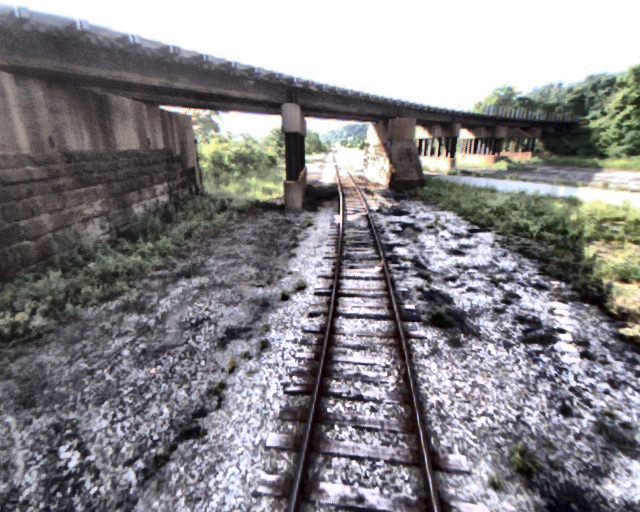
\includegraphics[scale=0.25]{images/clahe}
    \caption{Illumination Equalized using Clahe}
  \end{figure}

  
\end{itemize}
\end{document}
